%% LaTeX2e class for student theses
%% sections/evaluation.tex
%% 
%% Karlsruhe Institute of Technology
%% Institute for Program Structures and Data Organization
%% Chair for Software Design and Quality (SDQ)
%%
%% Dr.-Ing. Erik Burger
%% burger@kit.edu
%%
%% Version 1.3.5, 2020-06-26

\chapter{Regression}
\label{ch:Regression}

After extracting features from the elements, the next step is do learn from the data.
The goal of this Bachelor's thesis is to predict the activation barrier of a catalyst molecule.
The techniques used however are not limited to the activation barrier, 
as it can be expected that other properties of the molecule could be predicted with similar techniques.

For regression, artificial neural networks(ANNs) will be used.
Neural networks have seen a huge surge in popularity in recent years for their ability to 
adapt to high dimensional input data.
The concept is derived from biological neural networks such as the ones found in the human brain.

ANNs are a composed of a set of interconnected neurons.
Each neuron has a set of inputs $x_1 .. x_n$, a bias $b$, and an activation function $f(x)$.
The output will be the result of the activation function applied to the sum of all inputs plus the bias.

$$ y = f \left( \sum_i x_i + b \right) $$

Neurons are grouped together in layers, where the output of each layer is connected to the input of the next one.
For a single prediction, the example is applied to the input layer, the network is then flooded until the output layer is reached.
In the case of regression used here, the value of the output layer is the prediction of the neural network.

% Listing 2: Tex for neural network pipeline
\begin{tikzpicture}[
    % define styles    
    init/.style={ 
         draw, 
         circle, 
         inner sep=2pt,
         font=\Huge,
         join = by -latex
    },
    squa/.style={ 
        font=\Large,
        join = by -latex
    }
]
% Top chain x1 to w1
\begin{scope}[start chain=1]
    \node[on chain=1] at (0,1.5cm)  (x1) {$x_1$};
    \node[on chain=1,join=by o-latex] (w1) {$w_1$};
\end{scope}
% Middle chain x2 to output
\begin{scope}[start chain=2]
    \node[on chain=2] (x2) {$x_2$};
    \node[on chain=2,join=by o-latex] {$w_2$};
    \node[on chain=2,init] (sigma) {$\displaystyle\Sigma$};
    \node[on chain=2,squa,label=above:{\parbox{2cm}{\centering Activation\\ function}}]   {$f_{act}$};
    \node[on chain=2,squa,label=above:Output,join=by -latex] {$y_{out}$};
\end{scope}
% Bottom chain x3 to w3
\begin{scope}[start chain=3]
    \node[on chain=3] at (0,-1.5cm) 
    (x3) {$x_3$};
    \node[on chain=3,label=below:Weights,join=by o-latex]
    (w3) {$w_3$};
\end{scope}
% Bias
\node[label=above:\parbox{2cm}{\centering Bias \\ $b$}] at (sigma|-w1) (b) {};
% Arrows joining w1, w3 and b to sigma
\draw[-latex] (w1) -- (sigma);
\draw[-latex] (w3) -- (sigma);
\draw[o-latex] (b) -- (sigma);
% left hand side brace
\draw[decorate,decoration={brace,mirror}] (x1.north west) -- node[left=10pt] {Inputs} (x3.south west);

\end{tikzpicture}



% Listing 1: Tex for neural network layers
\begin{tikzpicture}[
    % define styles 
    clear/.style={ 
        draw=none,
        fill=none
    },
    net/.style={
        matrix of nodes,
        nodes={ draw, circle, inner sep=10pt },
        nodes in empty cells,
        column sep=2cm,
        row sep=-9pt
    },
    >=latex
]
% define matrix mat to hold nodes
% using net as default style for cells
\matrix[net] (mat)
{
% Define layer headings
|[clear]| \parbox{1.3cm}{\centering Input\\layer} 
   & |[clear]| \parbox{1.3cm}{\centering Hidden\\layer} 
   & |[clear]| \parbox{1.3cm}{\centering Output\\layer} \\
        
$\alpha_{0}^{0}$  & |[clear]|        & |[clear]| \\
|[clear]|         & $\alpha_{0}^{1}$ & |[clear]| \\
$\alpha_{1}^{0}$  & |[clear]|        & |[clear]| \\
|[clear]|         & |[clear]|        & |[clear]| \phantom{$a_{0}^{0}$} \\
$\alpha_{2}^{0}$  & $\alpha_{1}^{1}$ & $\alpha_{0}^{2}$ \\
|[clear]|         & |[clear]|        & |[clear]|  \phantom{$a_{0}^{0}$} \\
$\alpha_{3}^{0}$  & |[clear]|        & |[clear]| \\
|[clear]|         & $\alpha_{2}^{1}$ & |[clear]| \\
$\alpha_{4}^{0}$  & |[clear]|        & |[clear]| \\ 
};
% left most lines into input layers
\foreach \ai in {2,4,...,10}
   \draw[<-] (mat-\ai-1) -- +(-2cm,0);
% lines from a_{i}^{0} to each a_{j}^{1}
\foreach \ai in {2,4,...,10} {
   \foreach \aii in {3,6,9}
       \draw[->] (mat-\ai-1) -- (mat-\aii-2);
       }
% lines from a_{i}^{1} to a_{0}^{2}
\foreach \ai in {3,6,9}
 \draw[->] (mat-\ai-2) -- (mat-6-3);
   
% right most line with Output label
\draw[->] (mat-6-3) -- node[above] {Output} +(2cm,0);
\end{tikzpicture}

Finding the right amount of layers and the right type of activation functions is a challenging part of neural network.
Since generally no rule is known on what neural network architecture will work best on the given data, the sapce of possible networks needs to be explored.
A variety of choices for the network architecture can be made, such as the amount of layers, size of the layers, type of activation functions, regularization, normalization, and many more.

When choosing the network architecture, generally a bigger network will be able to adapt to the data better.
However if the network will become to big, it might encounter issues with overfitting.
Overfitting is a problem encountered when the network adapts to the training data too well.
This will decrease it's chances to generalize the data and make predictions on previously unseen samples \ref{fig:overfitting}.

\begin{figure} [h]
    \centering
    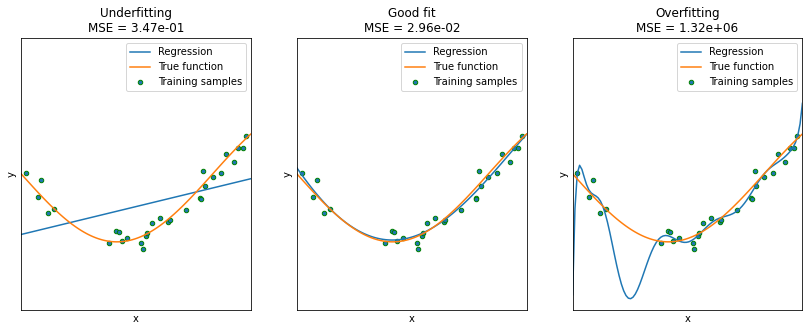
\includegraphics[width=0.9\textwidth]{figures/regression/overfitting.png} 
    \caption{Regression on a function with training examples. 
            The underfitting model is not complex enough to fit to the data well. 
            The overfitting model is too complex for the data.
            While the training error is lower for the overfitting model, 
            the overall performance of the overfitting model on previously unseen data 
            is worse than for the model with a good fit.
        }
    \label{fig:overfitting}
\end{figure}
  
To prevent overfitting while still getting good regression results, multiple network architectures need to be considered.
The networks proposed here were found by trail and error first, and later improved by hyperparameter analysis.

%TODO: Introduce NNs, normalzation, regularization, overfitting, underfitting.
% TODO: Regularization
% TODO: Normaliztation blabla

\section{Regression on fourier descriptor features}
\label{sec:Evaluation:fourier}

In the first approach, the features generated by the fourier descriptor were used to training.
Notable hyperparameters to the feature extractor here are the number of layers $l$ and the order of the fourier descriptor $o$.

Other parameters, such as the start height of slices and cutoff radius are chosen so that all the elements in 
the dataset full fit into the limitations.

The output shape of the descriptor will be an array of size $l \times o$.
Generally, the bigger the number of fourier coefficients, the better the contour can be approximated.
The same goes for the amount of layers. 
The more layers are chosen, the higher the sampling rat of the model and therefor the more accurate the representation.

This creates a tradeoff between accuracy and dimensionality.
Since neural networks are generally able to learn better from lower dimensional input spaces, 
a balance has tro be found between sufficiently approximating the input data and keeping the 
dimensions low enough to allow the neural network to learn without to much overfitting.



Since every slice is composed of same kind of fourier coefficients, the first idea was to use convolution layers the decrease the dimensionality of the input.
Filters might be able to recognize structures in each of the slices, and applied them across the different slices.

Convolution layers heavily depend on the assumption that the relative location of features in matters.
Filter sizes were therefor chosen to correspond to the dimensions over which similarities in the structures of the features are expected.
In the case of fourier coefficients, the filter therefor were only stretched along the layer dimension, and not along the dimension of the fourier descriptors.

In the first tests, the network was overfitting significantly.
Overfitting is a strong indication that the features generated by the features generator are sufficient to learn from them.
However due to the strong overfitting, the prediction results on previously unseen test data were much worse.

To get hold of overfitting, regularization was introduced.
Regularization punishes the model for extreme values and therefor reducing the amount of overfitting.

With several regularization techniques the test error could be reduced significantly. 
The overall accuracy however was by a factor of XXX worse than the models proposed in \cite{friederich_dos}.

In attempt to improve classification accuracy the SNAP feature extractor was developed.

\section{Regression on SNAP features}
\label{sec:Evaluation:snap}

Similar to the feature space for fourier coefficients, the size of the SNAP feature space is determined by two factors.
The first is the number of elements in the dataset.
The second is the resolution of the encoding for each type of element, defined by $n_{max}$ and $l_{max}$.

While the number of elements is fixed by the elements appearing in the dataset, $n_{max}$ and $l_{max}$ are hyperparameters that need to be choosen manually.
$n_{max}$ and $l_{max}$ also influence the resolution of the reconstruction of the element.
A plain hyperparamter optimization is therefor not viable, since the main objective in the end
is to reconstruct the 3d space to identify the areas important to the prediction.

A good balance between interpretability and accuracy was found with $l_{max}=n_{max}=3$. 
The network architecture and hyperparameter optimization will therefor be focused on these values.

\subsection{Normalization}

In a first step, the features generated by SNAP and the labels were normalized.
Normalize means scaling both labels and features independently so that mean is equal to $0$ and the standard deviation is equal to $1$.
Normalization helps the network to better adapt to the data and improves network stability to noise in the input data.
% TODO: Ellaborate

\subsection{Convolutional Neural Network}



\section{Comparison}
\label{sec:Evaluation:Comparison}

\dots
%% ---------------------
%% | / Example content |
%% ---------------------